%!TEX root = ../template.tex
%%%%%%%%%%%%%%%%%%%%%%%%%%%%%%%%%%%%%%%%%%%%%%%%%%%%%%%%%%%%%%%%%%%
%% chapter1.tex
%% NOVA thesis document file
%%
%% Chapter with introduction
%%%%%%%%%%%%%%%%%%%%%%%%%%%%%%%%%%%%%%%%%%%%%%%%%%%%%%%%%%%%%%%%%%%

\typeout{NT FILE chapter3.tex}%

\chapter{Logic Tools}

In this section...

\section{Iltis Web-Based System for Teaching Logic}
\label{chap:iltis}
Iltis is an interactive online tool designed to help people learning logic from scratch.~\cite{arxivIltisLearning, arxiv} The goal of this tool is to provide a system that supports a wide variety of content (propositional logic, modal logic, and first-order logic) along with a valuable feedback system that helps the learner to better understand their mistakes. This web application is divided into multiple sections. Each section is comprised of a set of tasks (exercises) that increase in difficulty as the learner completes the exercises. For each kind of task, this application provides a custom feedback generator. This feedback can vary depending on the mistakes made by the learner. Some tasks have different levels of feedback that may differ based on the learner’s proficiency. Low feedback levels provide a vaguer hint, and the high ones a more precise and explicit hint. The image below provides a list of the currently available types of exercises in Iltis.

\begin{figure}[htbp]
    \centering
    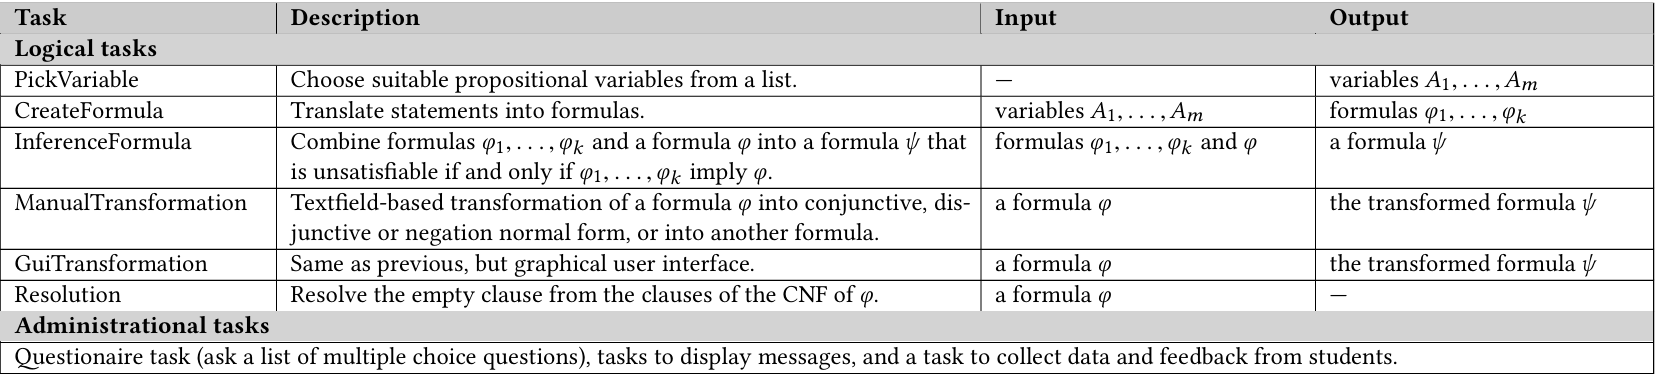
\includegraphics[width=1\linewidth]{Itils_list_of_tasks}
    \caption{List of tasks available in Iltis~\cite{arxiv}.}
\end{figure}

From the teacher’s perspective, this framework provides a way to create more tasks. Teachers can achieve this by using an XML file where they specify a set of tasks, the task type, and a list of feedback generators to be presented to the learner.

\subsection{Feedback}
\label{chap:iltis-feedback}
Iltis allows teachers to associate more than one feedback generator with the task, creating different levels of feedback. Some exercises have feedback generators constructed using reversion rules, providing better and more accurate feedback. In a previous study, researchers collected some of the most frequent mistakes made by learners and built a list of reversion rules. A common example of a reversion rule in the “Propositional Formulas” exercises is to switch the order of the antecedent and consequent in implications. Whenever a learner switches two parameters, the feedback generator tries to apply reversion rules to find the correct solution. If successful, this indicates that the solution is close to the correct one, making it possible to provide more precise feedback based on the applied rule(s). Otherwise, it suggests that the solution is far from the correct one.

\subsection{Conclusion}
There are some positive aspects to consider from this system when developing our own tool, such as the intuitive way (it presents a low learning curve, and it is fundamental for these kinds of tools) that the exercises are presented to the learner, the advanced feedback system, and the easy access to the tool. It also provides a vast set of exercise types and a modular way to create them. On the other hand, teachers need to specify tasks in XML, and this requires some extra knowledge. Some types of exercises are still missing in this tool, like the deduction tree proof. Additionally, this project was developed by a German university and is not open-source, so it cannot be used for further development or expansion.

\section{Logic4Fun}
Logic4Fun is an online tool with a wide range of logical problems and puzzles focused on logical modeling and formalization ~\cite{logic4fun}.
This tool was developed by an Australian university and has been in development since 2001. It was projected to help students practice and develop skills in formalizing logical problems, as this is a challenging topic to teach, and students often struggle with it.

Logic4Fun uses many-sorted first-order logic (MSFO) \footnote{Many-sorted first-order logic is an extension of first-order logic (FOL). In FOL, all variables 
come from the same domain limiting flexibility when modeling exercises with multiple distinct domains. MSFO extends this by allowing the assignment of types (or sorts) to variables and predicates, making the language more expressive.}language to express the problems. It has a solver that takes as input a set of formulas and searches for finite models of this set. This tool presents a web page with different levels of problems: Beginner, Intermediate, Advanced, Expert, and Logician, with increasing complexity. It starts with trivial exercises to help students better understand how to use the site (declare vocabulary, set constraints, and read the solver output) and progresses to more complex and challenging exercises that require a strong background in logic. One of the key advantages of using this tool is the ability to receive immediate and accurate feedback, in contrast with traditional teaching methods. This helps keep students motivated and encourages them to invest more time and effort into solving problems. This site also allows users to enroll in a course by using the credentials provided by the teacher.

\subsection{Feedback}
Logic4Fun tracks two kinds of errors: syntactic and semantic. Syntactic errors are mistakes in the structure or arrangement of words that violate the grammar rules of the language. These errors can be captured by the parser or type checker. When a user attempts to submit an exercise with syntactic errors, a message is presented with some suggestions. When the type checker detects an error, it provides more information, especially about the expected and provided types. Semantic errors are mistakes in logic or meaning in a programming language that occur in program execution. Since there are no predefined solutions, these errors are harder to classify and to deal with. Given these difficulties, Logic4fun simply indicates whether the solution is correct or not. To address the lack of feedback, they created a diagnostic tool to provide more informative responses to the users when a solution cannot be found. There are two approaches to give information provided by the diagnostic tool: using approximate models and using unsatisfiable cores.
\begin{itemize}
    \item In the approximate models approach, the solver starts by marking some unsatisfied constraints as "soft" and then attempts to satisfy as many as possible. Then a user can adjust constraints and rerun the solver, iterating to find the optimal approximations.
    \item In the unsatisfiable cores approach, the solver can try to identify groups of unsatisfied constraints that are causing the problem. Each group must contain at least one contradiction, giving useful clues for troubleshooting the problem. 
\end{itemize}

\subsection{Conclusion}
Logic4Fun has several positive aspects, such as allowing exercises to be saved, enabling users to pause their work and resume it later, progressively increasing the difficulty of exercises, helping users integrate with the tool, and incorporating a diagnostic tool to address the lack of feedback. It has a class system where professors can invite their students to enroll. However, it only provides a restricted range of exercises based on first-order logic. It has some limitations with the solver's performance (the number of models presented to the user is restricted), and it is still facing issues with feedback. Sometimes, the reported errors are overly detailed or unclear, which can become frustrating for the users.

\section{LOGAX}
LOGAX is a tool designed to help students in construction logic proofs in Hilber-style. [paper GENERATION andUseOfHintsandFeedback] This tool is capable of providing feeback and hints at different levels of the proofs. It can provide the solutions for the steps to follow, as well as the complete solution to the problem. 
Students are not strictly required to solve the exercises in one way, this tool allows proofs to be proven in both directions (bottom-up, top-down), as described in \ref{chap:prop-decution}. In deduction, there can be multiple possible solutions to the same problem. Based on the path followed by the user, LOGAX can adjust the solution space to better assist the user. This algorithm for adjusting the solution is based on the user's steps. If the user takes a step in the current solution space, LOGAX can give feedback and hints directly. However, if the step diverges from the solution space, it is necessary to recalculate it and then the system uses the new solution space to compute feedback and hints. This dynamic behaviour makes it possible to always offer feedback and hints to the user, ensuring they are not left lost in the exercise. 

 LOGAX has a system capable of automatically generating multiple possible solutions for a given proof. The algorithm is an adpatation of the one created by Bolotov ([Bolotov's Algorithm]). Bolotov's algorithm constructs a directed acyclic multigraph (DAM) from a list of premises and a conclusion. This data structure can captures all possible steps throughtout the proof that can lead to the conclusion. In this DAM, vertices represent statements and edges represent the rules. An example of a generated DAM in LOGAX is shown in imageX, where three assumption are given (\(p\), \(p \to q\) and \(q \to r\)) and the goal is to proof \( q \to r \vdash (p \to q) \to (p \to r) \). Edges correspond to rule applications: solid red edges represent the application of Modus Ponens (equivalent to the Implication Elimination rule) and dashed blue edges represent the application of the Deduction Theorem (equivalent to the Implication Introduction rule). Statement \((q \to r) \to (p \to (q \to r)) \) and \( p \to (q \to r) \to ((p \to q) \to (p \to r)) \) are axioms. This generated DAM captures tree different solutions for the same proof: one that uses axiom \(a\) and \(b\), one that uses the Deduction Theorem and axiom \(a\) and one that uses no axioms and applies the Deduction Theorem twice. 

\begin{figure}[htbp]
    \centering
    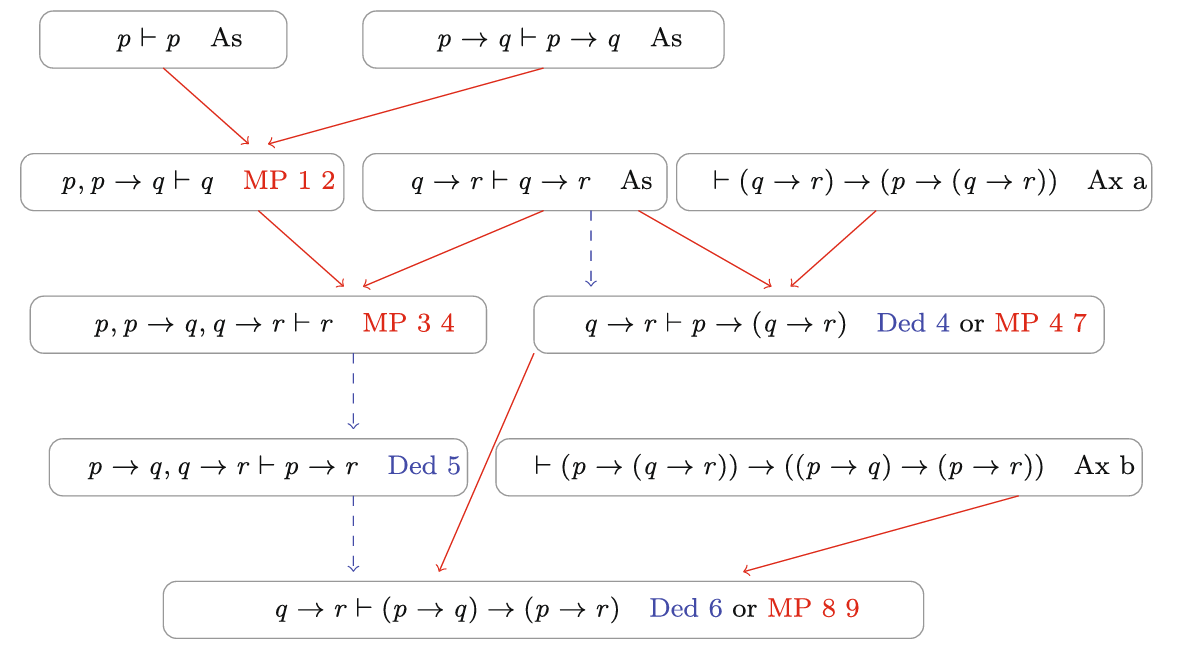
\includegraphics[width=1\linewidth]{LOGAX_DAM}
    \caption{Example of a directed acyclic multigraph generated by LOGAX.}
\end{figure}

Storing this information in a DAM makes it easier to provide feedback about the steps required to completed the proof at any given level. The user is not restricted to apply the rules in a specific order, the system can adapt to the user's solution if it divirges, simply by following the sequence of rules chosen by the user. This allows the system to easily provide information about next steps (top-down proof) or previous steps (bottom-up proof) using the edges. To provide a complete solution to the user, it is necessary to extract and trim the solutions from the DAM. 

The design of this tool focuses on interfaces that allow students to concentrate on the goal of solving proofs, rather than wasting time figuring out syntatic errors. Shortening the number of steps required and distractions to reach the goal leads to better learning outcomes.

\subsection{Hints \& Feedback}
Before developing the system, the LOGAX team explored two approaches to constructing guidance and providing feedback for a proof. One approach involves having a hidden solution, which can be provided by the teacher or derived from a set of student solutions. Howecer, this method has some drawbacks: it can only recognize solutions that are nearly identical to the stored proofs, it is limited to a fixed set of exercises, and every time a teacher wants to add a new exercise, they must provide a hidden solution. The second approach relies on the Bolotov's algorithm, which addresses all the isseus of the previous method.

After that, they began by developing a basic hint system that includes hints to: provide directions for the next steps (forward or backward), indicate the next rule to be applied, and offer an explicit step-by-step procedure for performing the next step. Then, after some studies, they realized that students exposed to informative feedback along with information about a subgoal are more likely to succeed in correcting mistakes than students exposed to only informative feedback. 
By providing feedback that includes information about subgoals, the system can help students understand why a certain step is useful. Consequently, the system was expanded to track a list of subgoals, in this case, sub-proofs while running the proof algorithm. This way, it can provide hints about subgoals at any level of the proof.

They also made some studies on students common mistakes on this kind of proofs and they came up with the following types of mistakes:
\begin{itemize}
    \item Oversights: Correspond to syntatic errors, for example, when a user forgets to close a parenthises in a sentence, or or when logical symbols are not placed in the correct position.
    \item Conceptual errors: Occurs when a student fundamentally misunderstands a concept or how it should be applied. For example, this error can occur when choosing the statements to apply a certain rule.
    \item Creative rule adaptations: Occurs when students try to invent their own rules. For example, from this \( \neg p \to (q \to \neg r) \) and \( q \), concluding \( \neg p \to \neg r \) using Modus Ponens(Implication Elimination rule). This usually happens when the student does not know how to proceed.
\end{itemize}

Finally, they expanded the system to also track those mistakes. This way, the system can point out a mistake and, if possible, mention exactly which formula, subformula, or set of formulas does not match the chosen rule.

\subsection{Conclusion}
LOGAX seems to fit perfectly with what is intended to be implement during this thesis for the deduction tree exercises (REF deduc tree exercises). It covers a wide rage of aspects to consider when developing a system like this. Starting with the algorithmn that finds all the possible solutions for a given proof, the fact that it ignores the order of the steps, and the ability to adjust the guidance based on the user's solution. It also includes different approaches for giving feedback and hints, as well as the idea of given subgoals as a hints to help the student understand the proof. Additionally, there are some important aspects regarding the design of the interfaces. 
Unfortuntly, this was an old project, and the tool is no longer available. This tool has some minor drawbacks that we can consider when developing our solution. One of them is the that the system doesn't provide fading strategies to reduce the amount of feedback. We might want to controll the amount of feedback sent to the student based on their level of expertise. Another problem this tool faces, is that the user can't erase lines of the proof. As a consequence, the final proof can be more extensive than expected. Overall, it seems to meet all the requirements for a good tutoring tool and for sure, this tool will be used as refence for the one that we are going to develop.

%\section{Iltis}
%\subsection{Conclusion}
